\documentclass[12pt,a4paper]{report}
\usepackage[utf8]{inputenc}
\usepackage{amsmath}
\usepackage{amsfonts}
\usepackage{amssymb}
\usepackage{graphicx}
\usepackage{caption}
\usepackage{svg}
%\usepackage{gensymb}
\usepackage{fourier}
\usepackage[francais]{babel}

\usepackage[top=2.5cm,bottom=2.5cm,right=2.5cm,left=2.5cm]{geometry}

\usepackage{url}
\usepackage{moreverb}
%\usepackage{multirow}
%\author{LEJEUNE Raphaël}
%\title{Titre}

\usepackage[fpms]{umons-coverpage}
\umonsAuthor{Raphaël \textsc{LEJEUNE} \\ Maximilien \textsc{POTTIEZ}}
\umonsTitle{Un robot contrôlé via un Raspberry Pi}
\umonsSubtitle{Projet d'informatique}
\umonsDocumentType{Rapport de projet}
\umonsSupervisor{Sous la direction de Monsieur le Professeur\\ Mohammed \textsc{BENJELLOUN}}
\umonsDate{2015}

\begin{document}

\umonsCoverPage

\tableofcontents

\chapter{Introduction}

Décrire le but visé, l'utilité du robot.

Faire en français et en anglais !

\begin{figure}[hf!]
\center
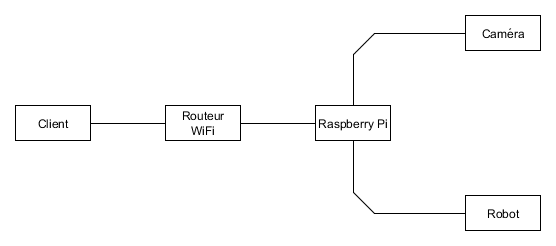
\includegraphics[scale=0.6]{GraphMateriel.png}
\caption{Matériel}
\end{figure}

\chapter{Matériel}

Lister le matériel utilisé, justifier sa présence

- Raspberry (pourquoi pas un Arduino, par exemple ?)
- Moteurs (quel modèle ?)
- Contrôleur (expliquer son utilité)
- Batterie
- Clé wifi
- Webcam (caractéristiques techniques)
- Réseau Wi-Fi opérationnel
- ?

\chapter{Software}

%Trouver un autre titre !!!

%Ici expliquer le principe des signaux PWM, des sockets, du multi-thread (même si pas utilisé... Parler des pistes envisagées)

%Captures d'écran

Lors de la réalisation du projet, nous avons envisagé plusieurs pistes pour contrôler le robot. 

\section{Signaux PWM}

Pour contrôler les moteurs, nous pouvons utiliser les signaux PWM (\textit{Pulse Width Modulation}) : il s'agit d'ondes carrées périodiques. 

Pour chaque période, on envoie une tension continue de 5 volts (qui correspond à la tension de base du Raspberry Pi, délivrée sur les ports GPIO) pendant une fraction de la période seulement. La tension « perçue » par le moteur est directement proportionnelle à cette fraction. Si cette fraction vaut par exemple 60 \%, le moteur tournera comme si on envoyait 3 V, donc à 60 \% de son régime maximum, si sa tension nominale est de 5 V. 

\chapter{Organisation}

\begin{figure}[hf!]
\center
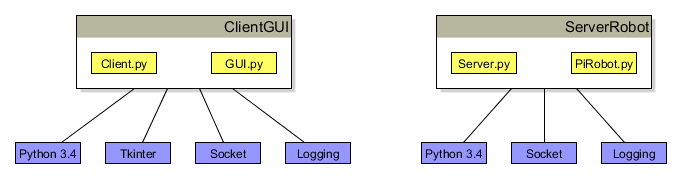
\includegraphics[scale=0.6]{GraphLogiciel.png}
\caption{Logiciel}
\end{figure}

Notre code est divisé en trois parties :

\bigbreak

\begin{itemize}
\item La partie client, qui tourne sur un PC (sous Windows, Linux, ...),
\item La partie serveur, qui se trouve sur le Raspberry Pi,
\item La partie contrôle, qui se trouve sur la carte Arduino.
\end{itemize}

\bigbreak

\paragraph{Client.py} sert à communiquer avec le Raspberry Pi. C'est dans ce fichier que sont récupérées toutes les requêtes de l'utilisateur, lorsqu'il appuie sur un bouton, par exemple.

\paragraph{GUI.py} sert à tracer l'interface graphique. Nous avons voulu créer des fonctions dans ce fichier et les lier directement au bouton comme ci-après :

\begin{verbatimtab}[3]
buttonstop = Button(frameRoot, text="STOP", command=buttonstopclick)
\end{verbatimtab}

Mais cela a entraîné des erreurs de références circulaires (car \textit{Client.py} dépend de \textit{GUI.py} et \textit{GUI.py} dépend de \textit{Client.py}). Nous avons résolu ce problème en ne donnant pas de fonction au bouton. Dans \textit{Client.py}, nous donnons explicitement la commande suivante :

\begin{verbatimtab}[3]
GUI.buttonstop.bind("<Button-1>", buttonstopclick)
\end{verbatimtab}

Cette seconde option présente deux avantages : on peut choisir le type d'événement à associer (bouton cliqué ou relâché, ...), et on peut aussi supprimer ce lien (avec la commande \verb=unbind=).

\paragraph{Server.py} est le programme qui tourne sur le Raspberry Pi. Son but est de recevoir les messages (depuis le client) et de les interpréter pour envoyer des instructions au robot.

\paragraph{PiRobot.py} est une classe qui contient toutes les fonctions d'envoi de commandes au robot, ainsi quand \textit{Server.py} reçoit un message, il n'a qu'à appeler la bonne fonction (par exemple la fonction \verb=Stop=, qui envoie une commande au robot pour arrêter les moteurs).

\paragraph{Python 3.2.3} est la version de l'interpréteur utilisé. Nous précisons ce détail, car certaines fonctionnalités que nous utilisons ne portent pas les mêmes noms dans d'autres versions de Python, ou n'existent tout simplement pas.

\paragraph{Tkinter} sert à tracer l'interface graphique. Il permet d'organiser assez facilement les éléments dans la fenêtre graphique.

\paragraph{Socket} permet d'ouvrir une connection entre une machine hôte (appelée Serveur) et une ou plusieurs machines (appelées Clients). Une fois la connection établie, les commandes \verb=send= et \verb=recv= permettent d'échanger des données.

\paragraph{Logging} sert à générer un fichier \text{.log}, contenant diverses informations. A titre d'exemple, la commande suivante est appelée dans la fonction \verb=buttonstopclick= :

\begin{verbatimtab}[3]
logging.debug('Button STOP click')
\end{verbatimtab}

Dans le fichier \text{.log}, on verra cette ligne :

\begin{verbatimtab}[3]
2015-07-28 18:06:08,051 root	DEBUG	Button STOP click
\end{verbatimtab}

C'est une alternative au \verb=print('Button STOP click')=, et qui permet de sauvegarder les actions faites lors de l'exécution d'un programme, même s'il est arrêté pour quelque raison que ce soit.

\paragraph{Github} est un système de contrôle de révision, et peut être utilisé pour plusieurs choses :

\begin{itemize}
\item Garder une copie des codes. C'est la raison principale. Si l'ordinateur ou le Raspberry rencontre un problème, le code est sauvegardé.
\item Il permet aussi d'enregistrer plusieurs versions d'un code, en montrant qui l'a mis en ligne, quand cela a été fait, et les différences avec la version précédente. C'est utile si on se rend compte que les modifications apportées à un code rend celui-ci inutilisable, en permettant de retélécharger un code qu'on sait fonctionnel. Sur la figure \ref{GitHub}, on voit que Sero17 (c'est le pseudo de Raphaël) a modifié le fichier \url{ClientGUI\GUI.py} il y a dix jours.

\begin{figure}[hf!]
\center
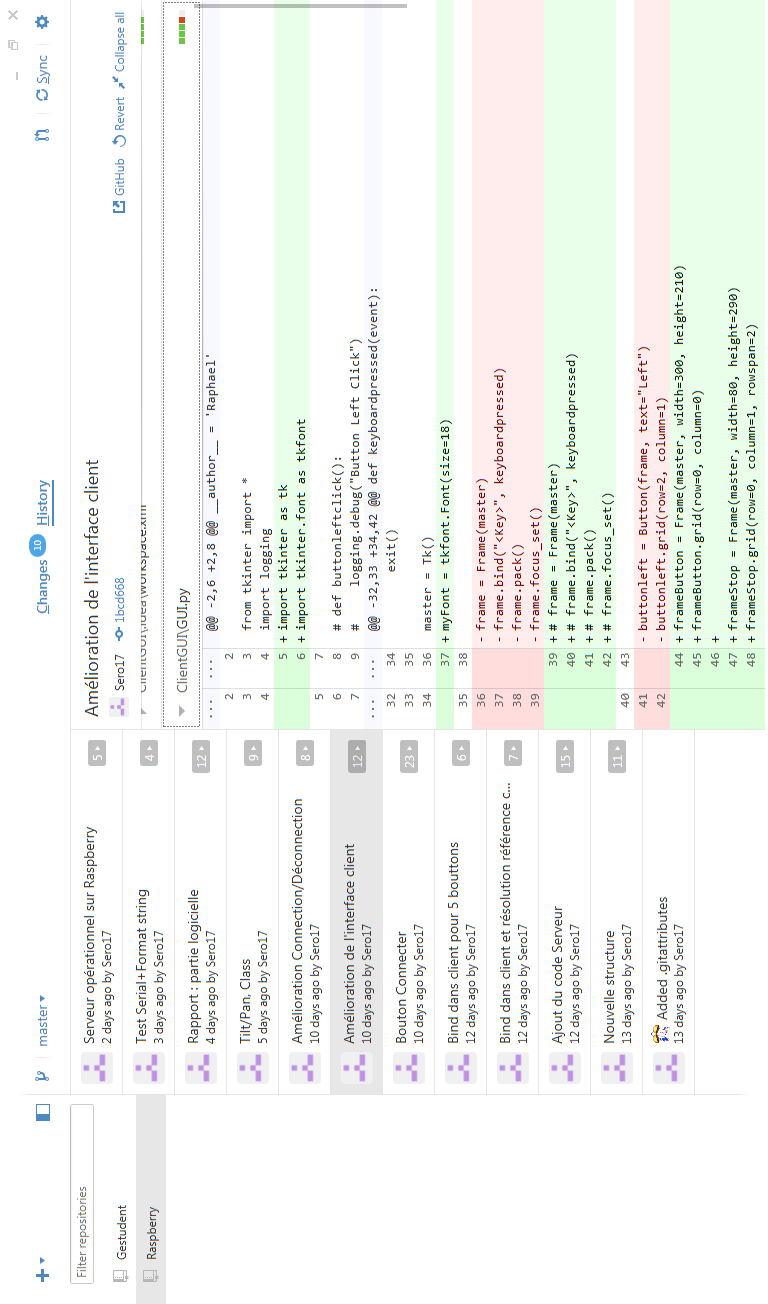
\includegraphics[scale=0.7]{GitHub.png}
\caption{Interface de GitHub sous Windows}
\label{GitHub}
\end{figure}
\end{itemize}

\chapter{Qui a fait quoi}

Raphaël

Recherches sur connection socket

Programme client, interface, programme serveur sur raspberry, connection serial avec arduino
Backup régulier des codes sur GitHub, ...

\chapter{Conclusion}

Difficultés rencontrées, limitations, améliorations possibles, ...

\appendix

\chapter{Procédure d'installation}

\section{Installation de Raspbian sur le Raspberry Pi}

Voici la procédure à suivre pour installer Raspbian sur le Raspberry :

\begin{itemize}
\item Téléchargez NOOBS sur \,\url{https://www.raspberrypi.org/downloads/}, et extrayez les fichiers du zip.

\item Formatez la carte SD (avec \,\url{https://www.sdcard.org/downloads/formatter_4/}). Sélectionnez la carte SD et dans les options choisissez \textit{FORMAT SIZE ADJUSTMENT ON}, puis cliquez sur \verb=Format=.

\item Copiez les fichiers extraits de NOOBS sur la carte SD, puis éjectez la carte et insérez-la dans le Raspberry Pi.

\item Connectez le Raspberry à un écran avec un câble HDMI, et connectez aussi un clavier et une souris sur les ports USB (un récepteur sans fil convient aussi).

\item Alimentez le Raspberry. Attention il est déconseillé de brancher/débrancher des câbles lorsque le Raspberry est sous tension. Si vous souhaitez changer l'écran ou un autre périphérique, éteignez d'abord le Raspberry et débranchez-le.

\item Sélectionnez Rasbian comme OS et la langue, ainsi que la configuration du clavier, et cliquez sur \textit{Installer}.

\item Après l'installation (compter environ 25 minutes), redémarrez le Raspberry Pi.

\item Dans les options proposées, choisissez \textit{Enable Boot to Desktop/Scratch}, et \textit{Desktop Log in as user 'pi'}. Ensuite dans \textit{Advanced Options}, choisissez \textit{SSH}, et \textit{Enable}. Allez sur \textit{Finish} (avec Tabulation) et redémarrez le Raspberry.

\item Si vous utilisez un écran avec un câble VGA et un adaptateur, il faut modifier \url{\boot\config.txt}. Il faut décommenter ou ajouter les lignes suivantes : 
\begin{verbatimtab}[3]
hdmi_force_hotplug=1
hdmi_group=2
hdmi_mode=69
hdmi_drive=2
\end{verbatimtab}
Le numéro 69 correspond à une résolution d'écran de 1920x1200, et une fréquence de 60 hz. Pour voir quel numéro correspond, voir \url{https://www.raspberrypi.org/documentation/configuration/config-txt.md}\, .

\item Configurez le WiFi (voir section suivante), et mettez à jour le système en entrant ces deux commandes :

\bigbreak
\begin{verbatimtab}[3]
sudo apt-get update
sudo apt-get upgrade
\end{verbatimtab}
\bigbreak

\end{itemize}



\section{Configurer le WiFi sur le Raspberry Pi}

Nous allons configurer le Raspberry pour se connecter au routeur, et lui assigner une IP fixe.

\begin{itemize}
\item Lorsque le Raspberry est hors tension, insérez la clé WiFi dans un port USB.
%\item Dans un terminal, entrez la commande \,\verb=ifconfig= pour récupérer ceci :
%
%\bigbreak
%\begin{verbatimtab}[3]
%wlan0	Link encap:Ethernet	HWaddr c4:a8:1d:7c:0b:60
%inet adr:192.168.1.104	Bcast:192.168.1.255	Masque:255.255.255.0
%\end{verbatimtab}
%\bigbreak
%
%\item Entrez ensuite \,\verb=sudo route -n=  :
%
%\bigbreak
%\begin{tabular}{lll}
%\verb=Destination= & \verb=Passerelle= & \verb=Genmask= \\ 
%\verb=0.0.0.0= & \verb=192.168.1.1= & \verb=0.0.0.0= \\ 
%\verb=192.168.1.0= & \verb=0.0.0.0= & \verb=255.255.255.0=\\ 
%\end{tabular}
%\bigbreak

\item Toutes les informations concernant le réseau peuvent être retrouvées grâce à un autre appareil connecté à ce réseau : entrez dans un terminal ces deux commandes :

\bigbreak
\begin{verbatimtab}[3]
sudo route -n
ifconfig
\end{verbatimtab}
\bigbreak

\item On édite un premier fichier de configuration : entrez cette commande : 

\bigbreak
\begin{verbatimtab}[3]
sudo nano /etc/wpa_supplicant/wpa_supplicant.conf
\end{verbatimtab}
\bigbreak

Ajoutez les paramètres du réseau Wi-Fi, et sauvegardez :

\begin{verbatimtab}[3]
network={
	ssid="<SSID du réseau local>"
	psk="<Clé de sécurité>"
	proto=RSN
	key_mgmt=WPA-PSK
	paiwise=CCMP
	auth_alg=OPEN
}
\end{verbatimtab}

\item On édite un autre fichier : entrez cette commande : 

\bigbreak
\begin{verbatimtab}[3]
sudo nano /etc/network/interfaces
\end{verbatimtab}
\bigbreak

Ajoutez les paramètres du réseau Wi-Fi, et sauvegardez :

\bigbreak
\begin{verbatimtab}[3]
auto lo

iface lo inet loopback
iface eth0 inet dhcp

allow-hotplug wlan0
auto wlan0

iface wlan0 inet static
address 192.168.1.50
netmask 255.255.255.0
broadcast 192.168.1.255
gateway 192.168.1.1
wpa-conf /etc/wpa_supplicant/wpa_supplicant.conf
iface default inet dhcp
\end{verbatimtab}
\bigbreak

L'adresse 192.168.1.50 est l'adresse IP que j'ai choisie pour le Raspberry. Il faut choisir une adresse en dehors de la plage d'adresse réservée pour le dhcp.

\item Réinitialisez le réseau avec ces deux commandes, ou redémarrez le Raspberry.

\bigbreak
\begin{verbatimtab}[3]
sudo ifdown wlan0
sudo ifup wlan0
\end{verbatimtab}
\bigbreak
\end{itemize}

\end{document}

